% GRASP: Copyright 1997,1998,1999  Bruce Allen
% $Id: man_timefrequency.tex,v 1.6 1999/11/23 23:27:40 ballen Exp $
\section{GRASP Routines: Time-Frequency Methods}
\label{s:tfmethods}
\setcounter{equation}0
This section describes the use of software written to extract signals
in noise via time frequency methods. Such methods will be useful in
extracting signals from poorly modeled or unmodeled sources.
The basic procedure we adopt involves the following steps,
\begin{itemize}
\item Construction of two dimensional 
`time-frequency' (TF) maps of the time series data,
\item Search for one-dimensional structures in the map. 
\item Use a statistic based on the length and/or the intensity of the
line to determine whether the structure is due to a signal.
\end{itemize}
Each of the above defined steps can be accomplished by various
algorithms. 
For a detailed discussion of one implementation of  
this strategy, please refer to \cite{timefreqpap} and references
therein. In this implementation we use the Wigner-Ville distribution
to construct the TF map and the Steger's line detection algorithm to
detect the line features in the map and a simple length threshold
to determine whether we have detected a signal.

In order to improve the computation/communication ratio during code
parallelization we introduce the concepts of segment and subsegment. 
The master process sends out large chunks of data called data segments.
Each data segment contains many subsegments  and the slave processes
compute the TF map for each subsegment in turn. The sizes of the
segments and the subsegments are user defined. Also some points at the
beginning and the end of each segments are not analysed. This can, of
course, be compensated for by padding. The number of points skipped
at the beginning and end are termed PRESAFETY and POSTSAFETY
respectively and are user defined.

\subsection{Construction of the TF map}
As mentioned earlier, there exist  many algorithms to construct a
 ``time-frequency'' map of a data stream. We have currently
 implemented three algorithms for the construction of the map. 
 We describe each of these below.

\subsubsection{Wigner-Ville Distribution}
\label{sss:WVD}
The Wigner-Ville distribution (WVD)  $\rho(t,f)$ is defined by the relation,
\begin{equation}
\label{eq:WigTrans}
\rho(t,f) = \int_{-\infty}^\infty h\left(t - \frac{\tau}{2}\right)
h^*\left(t + \frac{\tau}{2}\right) e^{2\pi i f\tau} d\tau,
\end{equation}
where $h(t)$ is the time series data. In practice we use the discrete
analog of the previous equation, 
\begin{equation}
   \rho_{jk} = \sum_{\ell=-N/2}^{N/2}~h_{(j-\ell/2)}~h_{(j+\ell/2)}
      ~e^{2\pi i k \ell/N}.
\end{equation}
This appears to presents a minor
dilemma, since (\ref{eq:WigTrans}) contains expressions of the form
$h(t-\tau/2)$, which when discretized become $h_{j-k/2}$. 
This implies that the original data has to be oversampled by at least
a  factor of 2. We resample our simulated data so
that $h_j\equiv h(2j\Delta t)$ accordingly. Among the various
algorithms to generated a TF map, we find that the WVD is most
suitable for our purpose. We show in figures \ref{f:wigwithoutsig} and 
\ref{f:wigwithsig} WVD distributions of timeseries data containing 
only noise and  timeseries data containing noise and an injected
signal. 
\begin{figure}[htbp]
\begin{center}
\epsfig{file=Figures/tfmap0.eps,angle=-90,width=3.2in}
\caption{ \label{f:wigwithoutsig}
The WVD of simulated initial LIGO noise.
 }
\end{center}
\end{figure}
The signal has been injected at an optimal filter signal to
noise ration of 8.

\begin{figure}[htbp]
\begin{center}
\epsfig{file=Figures/tfmap8.eps,angle=-90,width=3.2in}
\caption{ \label{f:wigwithsig}
The WVD of simulated initial LIGO noise and a signal embedded at an
SNR or 8.
 }
\end{center}
\end{figure}

Two versions of the Wigner-Ville transform are implemented. 
Equation (\ref{eq:WigTrans}) contains expressions of the form
$h(t-\tau/2)$, which when discretized become $h_{j-k/2}$. This implies
that for $j=0$ we require array points with negative indices. There
are two ways of handling this problem. One can assume that these array
points have a value of zero or one can assume that these array points
refer to data points before $h_0$. We implement both versions of the
Wigner transform. Please note that we have used the former one in 
\cite{timefreqpap}.

\subsubsection{Windowed Fourier transform}

The basic idea here is to multiply the data train with a window
function and compute the Fourier transform. We use the Welch Window
for our Windowed Fourier transforms (WFT). The WFT is defined by the
relation,
$$
\rho(t,f) = \int_{-\infty}^\infty h(\tau) w(\tau - t) e^{2\pi i f\tau} d\tau, 
$$
where, $w(t,\tau)$ is given as,
\begin{eqnarray}
w(\tau) &=& 1.0 - \frac{4.0 \tau^2}{d^2}  \ \ \ \ \ \  : \|\tau\| < d/2\\
&=& 0.0 \ \ \ \ \ \ \ \ \ \ \ \ \ \ \ \ \ \ \ \ \ :  \|\tau\| \geq d/2,
\end{eqnarray}

where $d$ is the width of the window. 

\subsubsection{Choi-William's distribution}
The Choi Williams distribution (CWD),  is given by the relation,
\begin{equation}
\rho(t,f) = \int_{-\infty}^\infty \int_{-\infty}^\infty h\left(u - \frac{\tau}{2}\right)
h^*\left(u + \frac{\tau}{2}\right) \sqrt{\frac{\pi\sigma}{\tau^2}}
e^{-\pi^2\sigma\frac{(u-t)^2}{\tau^2} - 2\pi i \tau f} d\tau du, 
\end{equation}
where $\sigma$ is the width of the window. As described in section
\ref{sss:WVD} we again need to oversample the data train at least by a
factor of two. Also it is to be noted that the Choi-Williams transform
is quite expensive to compute. 

\subsection{Steger's Line Detection Routines}
A gravitational wave signal in interferometer data $h(t)$ should produce a
ridge in the TFD $\rho(t,f)$.  Therefore, to detect GWs, a ridge detection
algorithm (or equivalently line detection algorithm if $\rho(t,f)$ is
represented as a gray-scale map as in Fig.  \ref{f:wigwithsig}) is required.
Fortunately, there are a number of ridge detection algorithms in the digital
image processing and computer vision literature from which to choose.

We use Steger's second-derivative hysteresis-threshold algorithm
\cite{Stegerspap}. The essential idea of this scheme is simple. A ridge in a
surface will have high curvature (second derivative of $\rho(t,f)$) in the
direction perpendicular to the ridge. Furthermore, the first derivative will
vanish at the top of the ridge, since it is a local maximum. Thus, ridges are
identified as contiguous sets of point at which $\rho(t,f)$ has a
high-curvature local maximum. We have included Stegers code
\cite{Stegerscode} in the GRASP package with minor changes. The main
aim of making the the changes was to enable Steger's routines to take
a map whose pixels are of type {\tt float} rather than {\tt unsigned
char}. For details about this algorithm please see \cite{timefreqpap,Stegerspap}





\newpage
\subsection{Structure: {\tt struct struct\_tfparam}}
\label{ss:tfstruct}
The structure  {\tt struct\_tfparam} is the main structure used by the
time-frequency routines and the program calling these routines. Some
of the fields of this structure are used by the time-frequency
routines while others are others are useful for book keeping. 
(We will use the abbreviation BK to denote the fields used for Book Keeping.) 

The fields of this structure are:\\
\noindent{\tt struct\_tfparam\{}
\begin{description}
\item {\tt int run\_number}: BK. An identification label. 
\item {\tt float f\_lower}: BK. The lower frequency cutoff for the
signals injected. 
\item {\tt int start\_segment}: BK. Used by the calling program to
identfy the first data segment to analyse.
\item {\tt int transformtype}: The type of the time-frequency
transform to be used to construct the map. Should be set to any one of
the three Macros defined in file grasp.h, namely, WIGNERTF,
WIGNERTF\_NP, WFFTWTF,
or CHOIWILLIAMS which correspond to the  
currently implemented transforms namely,the Wigner-Ville transform
with zero padding, Wigner-Ville transform without zero padding,
the windowed Fourier transform and  the Choi-Williams transform
respectively.
\item {\tt int windowidth}: The width (in number of  data points) 
of the window to use for the Choi-Williams and the windowed Fourier transform.
\item {\tt int offset\_step\_size}: 
This variable governs the resolution at which the TF map is computed
and should normally be
set to unity. If this variable is not set to unity then the
TF distributions are not computed for every value of time. For
example if this variable is set to 2 then the TF
distribution is computed at half the resolution.
\item {\tt int num\_of\_segments}: BK. The number of data segments to analyse. 
\item {\tt float maxpixelval}: Can be used to set a threshhold on
the values of the pixels in the TF map. This value can  be
computed using the routine {\tt compute\_scalefactor()}.
\item {\tt int DIM}: The data dimension of the data segment array.
\item {\tt int ND}: The data dimension of the subsegment array.
\item {\tt int PD}: The dimension of the TF map. Must be less that
ND/4.
\item {\tt int PRE}: The number of data points to skip at the beginning
of each segment. 
\item {\tt int POST}: The number of data points to skip at the end
of each segment.
\item {\tt int TD}: Has to be set to  ND/PD. 
\item {\tt int FD}: Has to be set to  ND/(4*PD)
\item {\tt float rescale\_factor}:  Used to compute maxpixelval via the routine 
{\tt compute\_scale\_factor()}. Has to be set to a number
greater than unity.
\item {\tt float hscale}: BK. An arbitrary scaling number. 
\item {\tt int noisetype}: BK. The type of noise. 
\item {\tt float srate}: The sampling rate.
\end{description}
{\tt \}}


\newpage

\subsection{Function: {\tt time\_freq\_map()}}

{\tt void time\_freq\_map(float *htilde, struct\_tfparam *tfs,int
index,float **tfgeneral,float **pic)}

This function is the main routine responsible for creating the
time-frequency map. Currently three algorithms are implemented for
creating TF maps from time series data, namely, the Wigner-Ville
distribution, the Windowed Fourier transform and the Choi-Williams
distribution. There are two versions of the  Wigner-Ville transform
which have both been implemented.  
This function calls the appropriate transform routine
based on the variabel {\tt (*tfs).transformtype}. 

The arguments are:

\begin{description}
\item {\tt float *htilde}: Input. The pointer to the beginning of the data
segment.
\item {\tt struct\_tfparam *tfs}: Input. A pointer to a structure
(defined in the previous subsection).
\item {\tt int index}: Input. The subsegment for which the map is
to be computed.
\item{\tt float **tfgeneral}: Input. A temporary work
space. Memory must be allocated by the calling program. {\tt tfgeneral} must
point to an array of size {\tt ((*tfs).TD * sizeof(*float))}. Each of these pointers must
be allocated a space of {\tt ((*tfs).ND * sizeof(float))}  bytes.
\item{\tt  float **pic}: Output. The computed TF map. Memory must
be allocated by the calling program. {\tt pic} must
point to an array of size {\tt ((*tfs).PD * sizeof(*float))}. Each of these pointers must
be allocated a space of {\tt ((*tfs).PD * sizeof(float))} bytes.
\end{description}

In addition to the arguments the structure variable {\tt (*tfs)} contains
all the additional parameters for the construction of the map. This
structure is defined in the previous subsection.

\noindent Author: R. Balasubramanian, bala@chandra.phys.uwm.edu

\subsection{Function {\tt compute\_scalefactor()}}

{\tt float compute\_scalefactor(float **pic,float rescale, int pdim)}

This function is used to compute the rescale value for the TF
maps. Such a rescaling is required for instance if the line
recognition algorithm requires input maps whose pixels are of type
unsigned char or short. It returns the maximum pixel value in the TF map multiplied by
the argument rescale. The arguments are:

\begin{description}
\item {\tt float **pic}: Input. The pointer to the TF map.
\item {\tt float rescale}: Input. The factor by which to multiply
the maximum pixel value.
\item {\tt int pdim}: Input. The size of the TF map. 
\end{description}

\noindent Author: R. Balasubramanian, bala@chandra.phys.uwm.edu

\newpage

\subsection{Function {\tt rescale()}}

{\tt void rescale(float **pic, int pdim, float rescale)}

This function is used to rescale and threshold TF maps so that the
pixel values lie between  zero and unity. The routine simply divides
each pixel by the argument rescale and sets any value greater than
unity to unity. Since the TF maps contain noise, it is possible for
the pixels to attain values which are much higher than the average.
To avoid losing information the argument rescale should  be obtained by
averaging the maximum pixel value in a large number of maps.
The routine {\tt compute\_scalefactor()} can be used for this purpose.
The arguments are:
\begin{description}
\item {\tt float **pic}: Input/Output. The pointer to the TF map.
\item {\tt int pdim}: Input. The size of the TF map. 
\item {\tt float rescale}: Input. The factor by which to divide
each pixel of the TF map.
\end{description}

\noindent Author: R. Balasubramanian, bala@chandra.phys.uwm.edu

\subsection{Function {\tt normalize\_picture()}}

{\tt void normalize\_picture(float **pic, int pdim)}

This function is used to normalize the TF map so that the pixel values
lie between zero and unity. In other words the maximum value is set to
unity and the minimum to zero and the rest of the values are scaled
uniformly. This function is useful since the routine {\tt plottf()}
requires the pixels of the TF maps to lie between zero and unity.
The arguments are:
\begin{description}
\item {\tt float **pic}: Input/Output. The pointer to the TF map.
\item {\tt int pdim}: Input. The size of the TF map. 
\end{description}

\noindent Author: R. Balasubramanian, bala@chandra.phys.uwm.edu


\subsection{Function {\tt gen\_quasiperiodic\_signal()}}

{\tt void gen\_quasiperiodic\_signal(float  *arr, int n, float fa, float
fs, float pind, float ampind, float timfrac, float freqfrac, int
*filled)}

This routine generates a quasiperiodic signal with both 
frequency and amplitude
increasing in time as power laws. The arguments are:
\begin{description}
\item {\tt float *arr}: Output. The array to contain the signal
points.
\item {\tt int n}: Input. The size of the data array.
\item {\tt float fa}: Input. The initial frequency of the signal. 
\item {\tt float fs}: Input. The sampling frequency.
\item {\tt float pind}: Input. The exponent for the power law increase
in frequency.
\item {\tt float ampind}: Input. The exponent for the power law increase
in amplitude.
\item {\tt float timfrac}: Input. The fraction of the length of
the data array for which the signal lasts.
\item {\tt float freqfrac}: Input. The fraction of the sampling
 frequency to be used as the upper cutoff frequency. Typically this
 should be around 15\% of the sampling frequency.
\item{\tt int *filled} Output. On return {\tt *filled } contains
the length of the signal.
\end{description}

\noindent Author: R. Balasubramanian, bala@chandra.phys.uwm.edu

\newpage

\subsection{Function: {\tt ppmprint()}}

{\tt void ppmprint(float **pic, char *file, int pdim)}

This function is used to print the TF map as a PPM format file. 
The arguments are:
\begin{description}
\item {\tt float **pic}: Input. The pointer to the TF map. The
pixel values must be between zero and unity.
\item {\tt char *file}: Input. A pointer to the name of the PPM
file. 
\item {\tt int pdim}: Input. The size of the TF map. 
\end{description}

\noindent Author: R. Balasubramanian, bala@chandra.phys.uwm.edu

\subsection{Function: {\tt pgmprint()}}

{\tt void pgmprint(float **pic, char *file, int pdim)}

This function is used to print the TF map as a PGM format file. 
The arguments are:
\begin{description}
\item {\tt float **pic}: Input. The pointer to the TF map. The
pixel values must be between zero and unity.
\item {\tt char *file}: Input. A pointer to the name of the PGM
file. 
\item {\tt int pdim}: Input. The size of the TF map. 
\end{description}

\noindent Author: R. Balasubramanian, bala@chandra.phys.uwm.edu

\subsection{Function: {\tt plottf()}}

{\tt void plottf(float **pic, int pdim)}

This function is used to print the TF map on the screen using GL/MESA calls.
The arguments are:
\begin{description}
\item {\tt float **pic}: Input. The pointer to the TF map. The
pixel values must be between zero and unity.
\item {\tt int pdim}: Input. The size of the TF map. 
\end{description}

\noindent Author: R. Balasubramanian, bala@chandra.phys.uwm.edu
\newpage

\subsection{Function: {\tt get\_line\_lens()}}
\label{ss:getlinelensfunc}
{\tt int get\_line\_lens(double sigma, double high, double low, int rows,
int cols, float **pic, char *file)}

This function detects one dimensional structures in the TF map. The
arguments are:
\begin{description}
\item{\tt double sigma}: Input. The width of the line to be
detected in pixels.
\item{\tt double high}: Input. The upper threshhold on the second
directional derivative.
\item{\tt double low}: Input. The lower threshhold on the second
directional derivative.
\item{\tt int rows}: Input. The number of rows in the TF map.
\item{\tt int cols}: Input. The number of columns. in the TF map.
\item {\tt float **pic}: Input. The pointer to the TF map.
\item {\tt char *file}: Input. The name of the file to which the
output is to be written. The file is written to disk only if at least one line is
detected in the map. The first entry in the file is the number of
lines detected. Then for each line detected the number of pixels in
the line and the sum of the TF map pixel values  along the line is recorded. 
A typical output file looks as shown below:

3\\
57 44.564186\\
24 10.698793\\
20 9.513889\\
\end{description}

\noindent Author: Warren G. Anderson, warren@ricci.phys.uwm.edu
This routine is an interface to the routines by Carsten Steger to
detect one dimensional structures in two dimensional images,
\cite{Stegerscode,Stegerspap}.

\subsection{Function: {\tt get\_lines()}}
{\tt int get\_lines(double sigma, double high, double low, int rows,
int cols, float **pic, float **out\_img)}

This function is almost identical with the function {\tt
get\_line\_lens()} defined in the previous subsection. The only
difference being the last argument of the function. The routine
returns a map ({\tt out\_img}) whose pixels have the value of either
unity if the pixel corresponds to a line point and zero otherwise.


\noindent Author: Warren G. Anderson, warren@ricci.phys.uwm.edu
This routine is an interface to the routines by Carsten Steger to
detect one dimensional structures in two dimensional images, 
\cite{Stegerscode,Stegerspap}.

\newpage

\subsection{Example: tfmain program}

This program was used to test the alogorithm described in the
Introduction (see section \ref{s:tfmethods}. We generate coloured
Gaussian noise and compute the TF map of each data subsegment and then
search for one dimensional structures in the map. The overall
structure of the code is as follows. We use
MPI code to set up a master slave operation. We have a single master
which generates data segments containing simulated Gaussian noise with
a signal embedded in the segment at an  SNR as specified in
the input file ({\tt tfmain.in}). Data segments containing only noise are
generated by setting SNR = $0.0$.
These segments are then passed on to the
slaves who compute the TF maps, detect the lines in each map and
write the output files directly to disk. In order to reduce the
communication overheads, the slaves compute many TF maps before they
request for more data. Each segment of data contains many subsegments
of data.  The slave computes the the TF map
and detects the lines therein for every subsegment in the segment
successively.

The program is divided into the following files:
\begin{description}
\item{\tt tfmain.h}: A header file containing function prototypes and
parameters.
\item{\tt tfmain.c}: The main program containing MPI code and
organizing the data flow.
\item{\tt tf\_get\_data.c}: Routines to  generate Gaussian random noise and
insert a signal at a given SNR.
\item{\tt tf\_misc.c}: Miscellaneous routines.
\item{\tt randomseeds}: Contains a single column  of random number seeds.
\item{\tt tfmain.in}: An input file containing various parameters read in by the program.
\item{\tt MergeSig.dat}: This file contains a single column of floating
point numbers and these are equally spaced samples of the coalescence
waveform for a pair of $30M_\odot$ blackholes. The sampling frequency
is 9868.4209 Hz. In addition we also include coalescence waveforms for
binaries in the mass range  $45M_\odot - 70M_\odot$. These files are
called {\tt MergeSig.dat.*} where * is a wildcard denoting the total
mass of the binary.
\item{\tt combine.c}: A program to combine the various output
files produced during a run. The original output files are deleted and
all the output information is written to a single file.
\item{\tt readertf.c}: A program to interpret the file produced by 
{\tt combine.c}. 
\end{description}

\subsubsection{Environment variables used by tfmain} 

The tfmain program uses the environment variable 
{\tt GRASP\_PARAMETERS}, the directory path which contains information
to construct the power spectrum for various detectors.

\newpage
\subsubsection{File: \tt tfmain.h}
\lgrindfile{Includes/tfmainh.tex}

\newpage
\subsubsection{File: \tt tfmain.c}
\lgrindfile{Includes/tfmain.tex}

\newpage
\subsubsection{File: \tt tf\_get\_data.c}
\lgrindfile{Includes/tf_get_data.tex}

\subsubsection{File: \tt tfmain.in}

This file acts as the input to the tfmain program. The routine
{\tt gettfparameters()} defined in the file {\tt tf\_misc.c}
reads in this input file. The file contains dummy strings describing the parameters
followed by that parameter. We list below the various input
parameters. The default values for the various parameters are the
ones used by us in investigating the efficiency of the algorithm
described in this section and is documented in \cite{timefreqpap}.
A run with these parameters reproduces the  point 
corresponding to the $60M_\odot$ curve at an SNR of 10 in Figure 5 of 
\cite{timefreqpap}. For convenience we reproduce the figure here, \ref{f:disvsmass}.
Please note that the parameters defined in file
{\tt tfmain.h} must also be unchanged to reproduce the results of our paper.
\begin{figure}[htbp]
\begin{center}
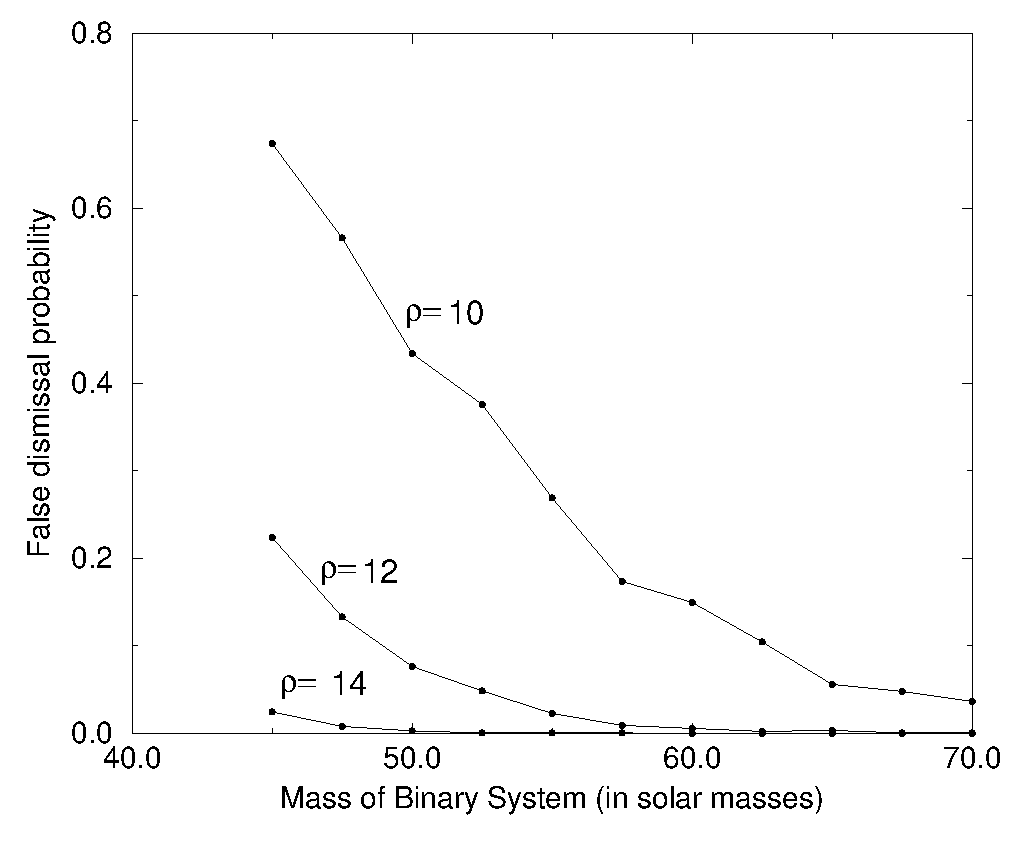
\epsfig{file=Figures/F_vs_M.eps,angle=0,width=3.2in}
\caption{ \label{f:disvsmass}
False dismissal probability as a function of mass. The three curves
correspond to three different values the optimal filter signal-to-noise ratio.
With the parameters we have chosen, our method tends to work better for higher
mass binaries, where the energy is more localized in the TF map.
 }
\end{center}
\end{figure}


\begin{description}
\item{\tt run\_number : } This is used when you need to make multiple runs
of the code for different parameters. The name of the directory to
write the output files is set to be {\tt ./run\$(run\_number)} where
{\tt \$(run\_number)} is the value of the parameter  run\_number. Also the 
random number seed used is determined by this number. The file
randomseeds contains a single column of user generated random numbers
which are used as seeds and the run\_number determines which random
seed to use and is essentially the random seed on the
run\_number$^{th}$ line in the file randomseeds.
\item{\tt flo : } This is the lower frequency cutoff for the generated
signal.
\item{\tt start\_segment : } the first segment to start analysing; segments
are numbered 0 onwards.
\item{\tt transform\_type : } To select between the Wigner-Ville(1), windowed
Fourier transform(2)  and Choi-Williams distribution (3), and
Wigner-Ville with no zero padding (4).
\item{\tt window\_width : } the size of the window used in the windowed
Fourier transform.
\item{\tt offset\_step\_size : } to be set to unity.
\item{\tt signal\_type : } the type of signal to insert in the
subsegments, inspiral waveform (1), quasiperiodic waveform with power
law increase in frequency and amplitude (2), coalescence waveform(3).
\item{\tt signal\_offset : } the offset at which to insert the signal in
each subsegment.
\item{\tt m1 : } mass of the star; used if  {\tt signal\_type  = 1}
\item{\tt m2 : } mass of the other star; used if  {\tt signal\_type  = 1}
\item{\tt pind : } the exponent for the power law increase in frequency;
used if {\tt signal\_type  = 2}
\item{\tt ampind : } the exponent for the power law increase in amplitude;
used if {\tt signal\_type  = 2}
\item{\tt timfrac : } the fraction of the subsegment for which the signal lasts;
used if {\tt signal\_type  = 2}
\item{\tt snr : } the signal to noise ratio at which to insert the signal
\item{number\_of\_segments : } the number of segments to analyse
\item{\tt dl\_sigma : } the value of the thickness of the lines expected
in the map in pixels.
\item{\tt dl\_high : } used as a threshold to determine whether a pixel is
part of a curve.
\end{description} 

\subsubsection{\texttt File:  {\tt combine.c}}

{\bf Usage: \tt combine directory\_name nseg nsubseg}\\
where  {\tt directory\_name} is the name of the directory containing the
output files of the {\tt tfmain} program {\em e.g.} run01. 
The argument {\tt nseg}
 is the number of segments which have been analysed. 
The argument {\tt nsubseg} is the number of subsegments in each segment of data.  

The program outputs a single file called {\tt allcurv.dat} in the
output directory. The format of the file is as follows. There is one
line for every subsegment analysed. The first number in each line is
simply an index from 0 to {\tt nseg*nsubseg - 1}. The next number in each
line is the number of lines detected and the subsequent numbers are
the number of pixels and the strength of each line in a alternating
sequence. The original output files are deleted.

\subsubsection{File: \tt readertf.c}
{\bf Usage: \tt readertf directory\_name}\\
where  {\tt directory\_name} is the name of the directory containing the
file {\tt allcurv.dat}.  This program reads this file and writes a new
file called {\tt curves.dat}. The basic purpose is to select the longest
line in each analysed subsegment. The format of the file is described
below. There is again one line for every analysed data subsegment. The
first column is an index ranging from 0 to the total number of data
subsegments analysed. The subsequent columns are, the number of curves
found, the length of the longest curve, the strength of the curve, and
the average strength for that curve respectively. 
The average strength is just the strength divided by the length.

